\documentclass[border=10pt, tikz]{standalone}
\usepackage{tikz}
\usepackage{fontspec}
\setmainfont{Songti SC}
\setsansfont{Heiti SC}
\usetikzlibrary{arrows.meta, positioning}

\begin{document}
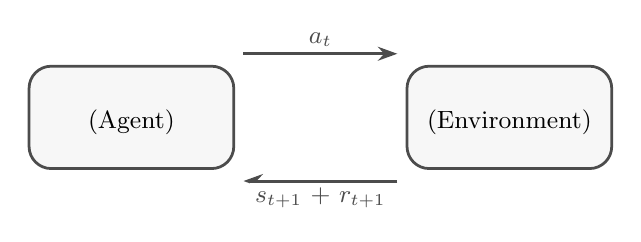
\begin{tikzpicture}[
    box/.style={
        draw=black!70, rounded corners=8pt, minimum width=2.6cm, minimum height=1.3cm,
        font=\normalsize, align=center, line width=1pt, fill=black!3
    },
    arrow/.style={
        -{Stealth[length=7pt, width=5pt]}, line width=1.1pt, black!70,
        shorten >=3pt, shorten <=3pt
    },
    lbl/.style={font=\small, text=black!70, fill=white, inner sep=2pt}
]

\node[box] (agent) at (0, 0) {\\[-2pt]{\small (Agent)}};
\node[box] (env) at (4.8, 0) {\\[-2pt]{\small (Environment)}};

\draw[arrow] ([yshift=4pt]agent.north east) -- node[above, lbl, pos=0.5] { $a_t$} ([yshift=4pt]env.north west);

\draw[arrow] ([yshift=-4pt]env.south west) -- node[below, lbl, pos=0.5] { $s_{t+1}$ +  $r_{t+1}$} ([yshift=-4pt]agent.south east);

\end{tikzpicture}
\end{document}
